\documentclass[11pt,a4paper]{article}
\usepackage[T1]{fontenc}
\usepackage[utf8]{inputenc}
\usepackage{lmodern}
\usepackage[margin=2.2cm]{geometry}
\usepackage{amsmath,amssymb,mathtools}
\usepackage{booktabs,tabularx,array,longtable}
\usepackage{xcolor}
\usepackage{tikz}
\usetikzlibrary{arrows.meta,positioning}
\usepackage{caption}
\usepackage{float}
\usepackage[colorlinks=true,linkcolor=blue!45!black,urlcolor=blue!45!black]{hyperref}

\DeclareMathOperator*{\argmax}{arg\,max}
\DeclareMathOperator*{\argmin}{arg\,min}
\DeclareMathOperator{\Reg}{Reg}
\newcommand{\R}{\mathbb{R}}
\newcommand{\1}{\mathbf{1}}
\newcommand{\W}{\mathcal{W}}
\newcommand{\Fr}{\mathcal{F}}
\newcommand{\Kx}{\mathcal{K}}
\newcommand{\Tr}{\mathcal{T}}
\newcommand{\code}[1]{\texttt{\detokenize{#1}}}
\newcommand{\keybox}[1]{\par\smallskip\noindent\fcolorbox{black!35}{black!4}{\parbox{\dimexpr\linewidth-2\fboxsep-2\fboxrule}{#1}}\par\smallskip}
\newcolumntype{L}{>{\raggedright\arraybackslash}X}
\let\olditemize\itemize
\renewcommand{\itemize}{\olditemize\setlength{\itemsep}{1pt}\setlength{\parskip}{0pt}\setlength{\parsep}{0pt}}
\let\oldenumerate\enumerate
\renewcommand{\enumerate}{\oldenumerate\setlength{\itemsep}{1pt}\setlength{\parskip}{0pt}\setlength{\parsep}{0pt}}
\setlength{\parskip}{3pt}
\setlength{\parindent}{0pt}
\captionsetup{font=small,labelfont=bf,skip=4pt}

\title{\vspace{-1.2cm}The path-aware SPO portfolio tree\\[2pt]\large What the pipeline in \texttt{main.py} and \texttt{run.py} does, precisely}
\author{}
\date{18 September 2026}

\begin{document}
\maketitle
\vspace{-1.5cm}
\begin{center}\small Code state: commit \texttt{36b2ffc} plus the uncommitted changes of \code{_best_split} (parent refit, largest regret reduction) and of \texttt{tests/test\_tree.py} (two new tests); 35 tests pass.\end{center}
\vspace{-0.2cm}

\keybox{\textbf{At a glance.}
\begin{itemize}
\item \textbf{Pipeline.} Daily closes and your daily features $\to$ one row per weekly decision $\to$ a decision tree whose leaves hold a \emph{predicted-return vector} $\to$ an exact portfolio optimizer with fees and a covariance penalty $\to$ weights. A replay trades the tree week by week, with drifting holdings and fees, and gives the Sharpe ratio.
\item \textbf{What is learned.} Leaf values minimise the \emph{decision regret} (SPO loss) of the portfolios they induce. Candidate splits are tried in decreasing order of regret reduction, and the first one that also raises the Sharpe ratio of the tree's own replayed path is accepted.
\item \textbf{Status.} The code does what it claims: 35 unit tests, 20 planted bugs all caught, and an audit (Section~\ref{sec:tests}). On synthetic crypto-like data, extra leaves always improve the training figures; on the test year their gain is small and hard to tell from luck, except when the signal is strong and the history long. \emph{No result in this report comes from real BTC or ETH data.}
\end{itemize}}

\section*{Overview and notation}

\begin{figure}[H]
\centering
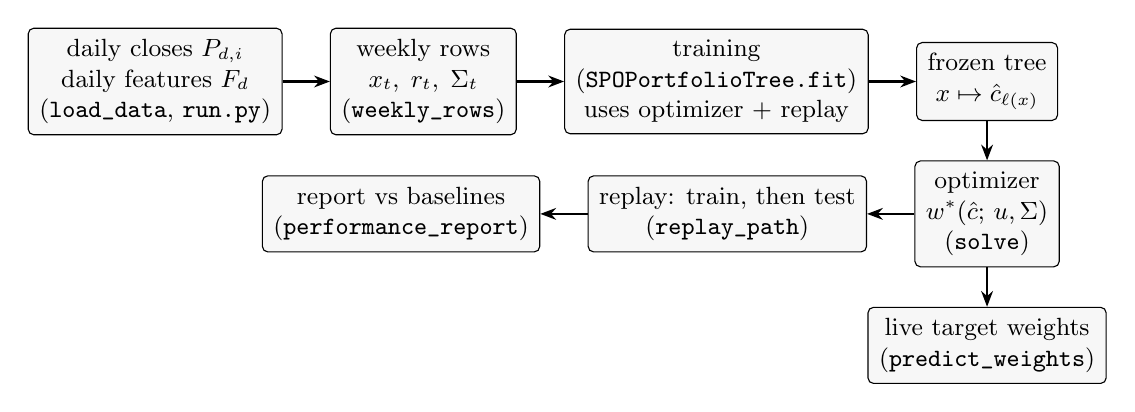
\begin{tikzpicture}[node distance=5mm and 6mm, every node/.style={font=\small},
  box/.style={draw, rounded corners=2pt, align=center, inner sep=4pt, fill=black!3},
  arr/.style={-{Stealth[length=2mm]}, thick}]
\node[box] (data) {daily closes $P_{d,i}$\\daily features $F_d$\\(\code{load_data}, \texttt{run.py})};
\node[box, right=of data] (rows) {weekly rows\\$x_t,\; r_t,\; \Sigma_t$\\(\code{weekly_rows})};
\node[box, right=of rows] (fit) {training\\(\code{SPOPortfolioTree.fit})\\uses optimizer $+$ replay};
\node[box, right=of fit] (tree) {frozen tree\\$x \mapsto \hat c_{\ell(x)}$};
\node[box, below=of tree] (opt) {optimizer\\$w^\ast(\hat c;\,u,\Sigma)$\\(\code{solve})};
\node[box, left=of opt] (replay) {replay: train, then test\\(\code{replay_path})};
\node[box, left=of replay] (report) {report vs baselines\\(\code{performance_report})};
\node[box, below=of opt] (live) {live target weights\\(\code{predict_weights})};
\draw[arr] (data) -- (rows); \draw[arr] (rows) -- (fit); \draw[arr] (fit) -- (tree);
\draw[arr] (tree) -- (opt); \draw[arr] (opt) -- (replay); \draw[arr] (replay) -- (report); \draw[arr] (opt) -- (live);
\end{tikzpicture}
\caption{The pipeline. \texttt{run.py} executes it end to end once \code{load_data()} is filled in.}
\end{figure}

\textbf{Abbreviations and sources.} \emph{SPO}: Smart Predict-then-Optimize, training a predictor on the quality of the decision it induces. \emph{SPOT}: Elmachtoub, Liang and McNellis, ``Decision Trees for Decision-Making under the Predict-then-Optimize Framework''. \emph{DIR}: Wang and Hasuike, ``Decision-Induced Ranking Explains Prediction Inflation and Excessive Turnover in SPO-Based Portfolio Optimization''. \emph{W--H SPO article}: Wang and Hasuike, ``Smart Predict--then--Optimize Paradigm for Portfolio Optimization in Real Markets''. \emph{DSPO}: Zhong et al., ``DSPO: An End-to-End Framework for Direct Sorted Portfolio Construction''. ``The Wang--Hasuike articles'' means DIR and the W--H SPO article.


\begin{table}[H]
\centering\small
\begin{tabularx}{\linewidth}{@{}l L l@{}}
\toprule
Symbol & Meaning & In the code\\
\midrule
$n$, $p$ & number of assets ($2\le n\le 4$, numbered from 0 as in the code) and of features & \code{n_assets}, \code{X.shape[1]}\\
$P_{d,i}$, $F_d\in\R^p$ & close of asset $i$ and feature vector on calendar day $d$ & \code{closes}, \code{daily_features}\\
$t=1,\dots,T$; $d_t$ & weekly decisions, and the day of decision $t$ & rows of \code{WeeklyRows}\\
$x_t$, $r_t$, $\Sigma_t$ & features, next-week simple returns, weekly covariance estimate & \code{X}, \code{R}, \code{Sigma}\\
$u_t$, $w_t$ & weights just before trading (holdings) and after trading & \code{holdings}, \code{weights}\\
$f\in\R^n_{\ge 0}$, $\lambda>0$, $\bar w$ & fee per traded notional (one value per asset), risk aversion, cap per asset & \code{fee_rate}, \code{risk_aversion}, \code{max_weight}\\
$c$, $\hat c_\ell\in[-b,b]^n$ & a predicted-return vector; the one stored in leaf $\ell$ & \code{prediction}, \code{prediction_bound}\\
$I_\ell$ & the training weeks that fall in leaf $\ell$ & \\
$\pi_t$, $S$ & net return of week $t$; Sharpe ratio per week & \code{net_returns}, \code{sharpe}\\
$\sigma^2$, $\varrho$ & weekly variance of an asset; correlation between two assets & \\
\bottomrule
\end{tabularx}
\caption{Notation. Weights are fractions of portfolio equity; returns are decimals ($0.01=1\%$).}
\end{table}

%=====================================================================
\section{What is the data?}\label{sec:data}

\subsection{What you supply}
\code{load_data()} in \texttt{run.py} is a stub that you fill in. It returns four objects:
\begin{itemize}
\item \code{dates}: consecutive calendar days, with no gap (crypto trades every day). A gap raises an error.
\item \code{closes}: a (days $\times$ $n$) array of positive daily closes, in the same asset order everywhere.
\item \code{daily_features}: a (days $\times$ $p$) array. Row $d$ must use information available at the close of day $d$ only. \code{NaN} is allowed on days that are not decision dates (the warm-up), never on a decision date. The first decision falls 180 to 186 days after the first close, so a feature with a longer look-back raises an error.
\item \code{current_weights}: your holdings now, for the live decision. They must be non-negative and sum to 1; \code{predict_weights} does not check it.
\end{itemize}

\subsection{From daily data to weekly rows}
{\small\emph{Code:} \code{weekly_rows}, \texttt{main.py:691}; \code{weekly_covariance}, \texttt{main.py:674}.}

A day $d$ becomes decision $t$ when it falls on the chosen weekday (default Monday), has $H=180$ daily returns behind it, and has a close seven days later. For each decision:
\begin{align}
r_{t,i} &= \frac{P_{d_t+7,\,i}}{P_{d_t,\,i}}-1, &
x_t &= F_{d_t}, &
\Sigma_t &= 7\,\widehat{\operatorname{Cov}}\big(q_{d_t-H+1},\dots,q_{d_t}\big)+\varepsilon I,
\label{eq:rows}
\end{align}
where $q_{d,i}=P_{d,i}/P_{d-1,i}-1$ is the daily return, $\widehat{\operatorname{Cov}}$ is the sample covariance (divisor $H-1$), and $\varepsilon=10^{-6}$ is a ridge. The factor 7 treats daily returns as independent and ignores compounding (a negligible understatement). \code{weekly_covariance} computes $\Sigma$ for one day; the live decision uses the same function, so training and trading share one estimator.

\begin{figure}[H]
\centering
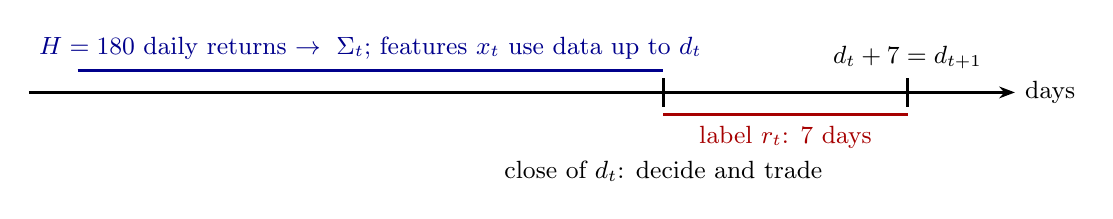
\begin{tikzpicture}[font=\small, x=0.62cm, y=1cm]
\draw[-{Stealth[length=2mm]}, thick] (0,0) -- (20.2,0) node[right] {days};
\draw[very thick, blue!55!black] (1,0.28) -- (13,0.28);
\node[above, blue!55!black] at (7,0.30) {$H=180$ daily returns $\to\ \Sigma_t$; features $x_t$ use data up to $d_t$};
\draw[very thick, red!65!black] (13,-0.28) -- (18,-0.28);
\node[below, red!65!black] at (15.5,-0.30) {label $r_t$: 7 days};
\draw[thick] (13,-0.18) -- (13,0.18); \node[below] at (13,-0.75) {close of $d_t$: decide and trade};
\draw[thick] (18,-0.18) -- (18,0.18); \node[above] at (18,0.18) {$d_t+7=d_{t+1}$};
\end{tikzpicture}
\caption{What one weekly row knows. Nothing to the right of $d_t$ enters $x_t$ or $\Sigma_t$.}
\end{figure}

\textbf{Timing.} Everything in $x_t$ and $\Sigma_t$ is known at the close of $d_t$; the label $r_t$ starts at that same close. The strategy is assumed to trade at that close. A unit test changes every price after a decision close and checks that the row's $x_t$ and $\Sigma_t$ do not move. \emph{Your features are not checked}: their causality is your responsibility.

\textbf{Sizes.} Five years of daily data (1,826 days) give 234 weekly rows; ten years give 495. \code{train_and_test} holds out the last 52 rows, so training has 182 or 443 rows. The label of the last training row ends exactly at the first test decision, so nothing overlaps.

\subsection{What is not in the data}
\begin{itemize}
\item \textbf{No cash.} Portfolios are fully invested ($\1^\top w=1$). A cash or stablecoin position can be added today as a constant-price column: the ridge keeps $\Sigma_t$ positive definite, and the unchanged code runs (checked). Give that column a zero fee, \code{fee_rate=(f, f, 0)}: with a scalar \code{fee_rate}, a move from a coin to cash is charged on both legs, $2f$, twice the cost of the single trade it really is.
\item \textbf{One asset is impossible}: the code needs $n\ge 2$, and with $n=1$ the only feasible weight is 1.
\item The weekly rows ignore the path inside the week, volumes (unless you put them in a feature), the risk-free rate, spreads and slippage.
\end{itemize}

%=====================================================================
\section{Features: nature, frequency and choice}\label{sec:features}

\textbf{The code prescribes no feature.} It only reads your array. The demo and the experiments use five: the 28-day momentum of assets 0 and 1, the 7-day momentum of asset 0, the 28-day volatility of asset 0, and a \emph{pure-noise column used as a control}. The Wang--Hasuike articles feed a linear model with daily technical indicators per asset: log return, moving average (10 days in DIR), price bias, RSI (14 days in DIR), MACD difference, Bollinger-band width and a volume indicator. That list is not a recommendation for a tree: a moving average of prices is a level (see below).

\subsection{What the pipeline does with a feature}
\begin{itemize}
\item \textbf{Frequency.} Features are computed daily from daily data, but only their value at the weekly decision close is used: one row in seven. The label is the return over the \emph{next seven days}. A look-back window of days to months is natural for that horizon.
\item \textbf{Only the ordering matters.} A split is $x_j\le\theta$, with $\theta$ halfway between two observed values. An increasing transformation of a feature (log, rank, scaling) gives the same partition of the training rows and the same leaf values, so no normalisation is needed. Only a new point that falls between the two training values around $\theta$ can be routed differently.
\item \textbf{The model is piecewise constant.} A tree of depth 2 has at most four leaves, hence four predicted-return vectors. Features should therefore describe \emph{states of the market} (regimes), not fine forecasts. Two nested splits capture an \emph{interaction} of two features, for example ``calm and rising'' against ``calm and falling''.
\item \textbf{Use stationary quantities}: returns, ratios, volatilities. A threshold on a price level has no meaning out of sample.
\end{itemize}

\subsection{Three constraints that should drive the choice}
\begin{enumerate}
\item \textbf{Every feature adds candidate splits, and the best candidate looks good by luck.} With 182 training rows and a minimum leaf of 20, each feature brings 143 thresholds, so five features give 715 candidate splits at the root. On data with no signal, the best of them still removes 10\% of the regret at $\lambda=1$ (Table~\ref{tab:gate}). Hence: few features (five or fewer), each with an economic reason. A pure-noise column is a cheap diagnostic, best used in a separate fit: in the demo it sits in the traded tree and wins the first split.
\item \textbf{With fully invested weights only differences matter.} Adding a constant to all predicted returns does not change the portfolio (Section~\ref{sec:decision}). With BTC and ETH only, a feature is useful exactly to the extent that it predicts $r_{\text{ETH}}-r_{\text{BTC}}$. Relative features (ETH/BTC momentum, relative volatility) are the direct candidates. Market-level features (BTC trend, volatility regime) can also qualify, because the two coins do not have the same beta. What they cannot do without a cash column is reduce the exposure to the market.
\item \textbf{A feature that crosses its threshold often creates trading.} Each change of leaf can move the whole portfolio and pay fees on both legs. In one earlier two-asset run ($\lambda=2$, fee 0.1\%, earlier split rule), 73\% (training) and 82\% (test) of the fees came from leaf changes that did not correspond to a change of regime. Persistent features (longer windows, moving averages of returns) reduce this.
\end{enumerate}

\textbf{Candidates for BTC and ETH, to be validated on real data:} momentum of each coin and of the ETH/BTC ratio over one to three months; realised-volatility regime; drawdown from the recent high; and, if the data is reliable, volume or funding-rate indicators. Real effects are likely to be interactions (a trend that works only in calm markets, for instance). That is the case a tree can represent and a one-feature rule cannot.

%=====================================================================
\section{What the tree learns: the decision problem, the regret and the Sharpe ratio}\label{sec:learn}

\subsection{The decision problem solved for every prediction}\label{sec:decision}
{\small\emph{Code:} \code{PortfolioOptimizer.solve}, \texttt{main.py:176}.}

Given a predicted-return vector $c$, holdings $u$ and a covariance $\Sigma$, the portfolio is
\begin{equation}
w^\ast(c;u,\Sigma)=\argmax_{w\in\W}\; c^\top w-f^\top|w-u|-\lambda\,w^\top\Sigma w,
\qquad \W=\{w\in\R^n:\ 0\le w_i\le\bar w,\ \1^\top w=1\}.
\label{eq:decision}
\end{equation}
With one fee for all assets and $\bar w=1$ this is equation~8 of DIR, with the holdings $u$ in the place of the previous portfolio; the code also allows one fee per asset and a cap. The optimizer is deterministic and is never trained.

\textbf{Exact solution.} At the optimum each weight is at $0$, at $\bar w$, at $u_i$ (fees put a kink there), or free strictly above or below $u_i$: $5^n$ patterns. Take a pattern with free set $\Fr$, fixed set $\Kx$ (its complement, with weights $w_\Kx$ fixed at $0$, $\bar w$ or $u_i$) and sides $s_i=\operatorname{sign}(w_i-u_i)$ for $i\in\Fr$. Stationarity under the budget constraint is a linear system:
\begin{equation}
A\,w_\Fr+\nu\1=g,\quad \1^\top w_\Fr=1-\1^\top w_\Kx,\qquad
A=2\lambda\Sigma_{\Fr\Fr},\quad g=c_\Fr-s_\Fr\circ f_\Fr-2\lambda\Sigma_{\Fr\Kx}w_\Kx,
\end{equation}
so $\nu=\big(\1^\top A^{-1}g-(1-\1^\top w_\Kx)\big)/\big(\1^\top A^{-1}\1\big)$ and $w_\Fr=A^{-1}(g-\nu\1)$. A pattern is admissible if all weights respect the bounds, every free weight lies on its assumed side of $u_i$, and, when no weight is free, the fixed weights sum to 1 (tolerance $10^{-9}$). Every admissible candidate is a feasible portfolio, and the one with the highest objective is returned (then clipped to $[0,\bar w]$). Since $f\ge0$, $\lambda>0$ and $\Sigma\succ 0$, the objective is strictly concave: the optimum is unique, and its own pattern reproduces it, so the enumeration is exact. All rows are solved in one vectorised call. The $5^n$ cost is why $n\le 4$.

\textbf{Properties that matter later.}
\begin{itemize}
\item \emph{Shift invariance:} $w^\ast(c+\alpha\1)=w^\ast(c)$. Only differences between predicted returns matter.
\item \emph{Two assets $a$ and $b$: closed form.} Let $v$ be the holding of asset $a$, $\Delta c=c_a-c_b$, $\phi=f_a+f_b$, $\kappa=2\lambda(\sigma_a^2+\sigma_b^2-2\sigma_{ab})$ and $\bar a=(\sigma_b^2-\sigma_{ab})/(\sigma_a^2+\sigma_b^2-2\sigma_{ab})$ the minimum-variance weight. With $D=\Delta c-\kappa(v-\bar a)$, the weight of asset $a$ is
\begin{equation}
w_a=\begin{cases} v & \text{if } |D|\le\phi \quad\text{(no trade)},\\[2pt]
\bar a+\dfrac{\Delta c-\phi\,\operatorname{sign}(D)}{\kappa} & \text{otherwise,}\end{cases}
\qquad\text{then clipped to }[1-\bar w,\ \bar w].
\label{eq:twoasset}
\end{equation}
(Checked against the solver on 2,000 random cases, to $10^{-14}$.) So a leaf acts through \emph{one} number, $\Delta c$; the response is linear with slope $1/\kappa$; and the no-trade band has half-width $\phi$ (0.2\% with the default fees).
\item \emph{Scale.} With equal variances $\sigma^2$, correlation $\varrho$ and no fees, \eqref{eq:twoasset} gives $w_a=\tfrac12+\Delta c/\big(4\lambda\sigma^2(1-\varrho)\big)$: the portfolio is all-in as soon as $\Delta c\ge 2\lambda\sigma^2(1-\varrho)$. With 8\% weekly volatility this gap is $0.51\%\times\lambda$ for $\varrho=0.6$ and $0.26\%\times\lambda$ for $\varrho=0.8$ (closer to BTC and ETH). At $\lambda=1$ almost any prediction gives an all-in portfolio.
\end{itemize}

\subsection{The loss: decision regret}
{\small\emph{Code:} \code{utility}, \texttt{main.py:168}; \code{_score_prediction}, \texttt{main.py:560}.}

The realised utility of a decision $w$ in week $t$, and the regret (SPO loss) of a prediction $c$, are
\begin{align}
U_t(w;r_t)&=r_t^\top w-f^\top|w-u_t|-\lambda\,w^\top\Sigma_t w, \label{eq:utility}\\
\Reg_t(c)&=U_t\big(w^\ast(r_t;u_t,\Sigma_t);\,r_t\big)-U_t\big(w^\ast(c;u_t,\Sigma_t);\,r_t\big)\;\ge 0. \label{eq:regret}
\end{align}
The first term is the best decision in hindsight, \emph{from the same holdings} $u_t$. Fees and the covariance penalty are inside the regret (DIR eq.~10): a prediction is judged on the objective the optimizer really maximises. The benchmark is a one-week oracle, as in the articles; it does not plan over several weeks. Numerically, a row regret below $-10^{-6}$ (\code{regret_tolerance}) aborts the fit; negative values between $-10^{-6}$ and 0 are set to zero.

\subsection{The path and the Sharpe ratio}
{\small\emph{Code:} \code{replay_path}, \texttt{main.py:301}; \code{_trade}, \texttt{main.py:350}.}

A sequence of predictions $c_1,\dots,c_T$ is traded in time order, starting from $u_1=\1/n$ (or from given holdings):
\begin{equation}
w_t=w^\ast(c_t;u_t,\Sigma_t),\qquad
\pi_t=r_t^\top w_t-f^\top|w_t-u_t|,\qquad
u_{t+1}=\frac{w_t\circ(1+r_t)}{1+r_t^\top w_t}.
\label{eq:path}
\end{equation}
Holdings \emph{drift} with returns between two decisions, so keeping a constant target also costs fees. The Sharpe ratio is $S=\operatorname{mean}(\pi)/\operatorname{std}(\pi)$ per week (divisor $T-1$, no risk-free rate). The replay also returns the regret~\eqref{eq:regret} of every week along the path.

\subsection{What the tree is supposed to learn}
The tree is a piecewise-constant map $x\mapsto\hat c_{\ell(x)}$. The leaf vector $\hat c_\ell$ is \emph{not} trained to forecast returns accurately. It is trained so that the portfolios $w^\ast(\hat c_\ell;u_t,\Sigma_t)$ have a small regret on the weeks of the leaf. DIR calls such values ``decision-inducing scores'': they need not be calibrated forecasts. Here they are searched inside $[-b,b]^n$; DIR instead clips its predictions to $\pm0.1$ after training.

\textbf{Link with SPOT.} SPOT's Theorem~1 says that the leaf mean of the realised vectors minimises the leaf's SPO loss when the optimal decision for that mean is unique (always true here). It extends to objectives $c^\top w-h(w)$ \emph{when all rows of a leaf share the same} $h$, that is, the same $u_t$ and $\Sigma_t$. Here they differ by row, so the mean is only a starting point. A numerical check agrees: no random candidate beats the mean when $u$ and $\Sigma$ are shared, and many do when either varies by row.

%=====================================================================
\section{How the tree is built and trained}\label{sec:tree}

\subsection{Fitting one leaf}
{\small\emph{Code:} \code{_fit_leaf}, \texttt{main.py:569}.}

For a leaf with rows $I_\ell$, with the holdings $u_t$ \emph{frozen} at the last replay of the current tree:
\begin{equation}
\hat c_\ell\approx\argmin_{c\in[-b,b]^n} L_\ell(c),\qquad L_\ell(c)=\sum_{t\in I_\ell}\Reg_t(c).
\label{eq:leaf}
\end{equation}
The search is deterministic:
\begin{enumerate}
\item Start from the leaf's mean return, clipped to $[-b,b]$. If a \emph{fallback vector} is given, evaluate it too and take it only if it is strictly better. The fallback is the refitted parent for a child, the leaf's own stored vector for a refit, and nothing for the root.
\item Run 3 passes (\code{search_passes}). In pass $k$, for each asset in turn, evaluate $G=7$ equally spaced values of that coordinate (\code{search_grid_size}) and move to the best one if it is strictly better. Pass~0 spans $[-b,b]$; pass $k\ge1$ spans the current best $\pm\,2b/(G-1)^k$, inside $[-b,b]$.
\end{enumerate}
With $b=0.10$ the windows are $\pm0.1$, $\pm0.033$ and $\pm0.0056$, and the final step is about $0.002$. One fit costs $2+3nG$ evaluations of $L_\ell$ (65 for $n=3$), each one vectorised solve over the leaf. Against a dense search, the result is within 0.03\% (median) of the best regret found, 2.1\% at worst; the plain mean is 0.8\% above (median).

\subsection{Growing the tree}
{\small\emph{Code:} \code{fit}, \code{_best_split}, \code{_shortlist} and \code{_refit_leaves} (\texttt{main.py}, lines 411, 488, 525 and 545).}

Growth is \emph{best-first}: one split per round, chosen among all leaves, because the holdings couple the leaves.

\keybox{\textbf{Algorithm.}
\begin{enumerate}
\item[0.] \textbf{Root.} Fit one vector on all rows as if every week started from equal weights. Replay the tree: this gives the holdings $u_t$ it would really have had, the hindsight utilities, and the Sharpe ratio $S$.
\item[1.] \textbf{For each leaf} with depth $<$ \code{max_depth} and at least $2m$ rows ($m={}$\code{min_samples_leaf}):
  \begin{enumerate}
  \item[a.] \emph{Parent refit.} Refit the leaf itself on the current holdings: $\hat c^{\,\text{refit}}_\ell$. It is only a yardstick and the children's fallback; it is never written into the tree.
  \item[b.] \emph{Screen.} For every feature $j$ and threshold $\theta$, give each child its clipped mean return and compute $Q=L_{\text{left}}(\bar r_{\text{left}})+L_{\text{right}}(\bar r_{\text{right}})$. Keep the \code{shortlist_size}${}=3$ smallest $Q$.
  \item[c.] \emph{Regret reduction.} For each shortlisted split, fit both children with~\eqref{eq:leaf} and compute
  $\Delta=L_\ell(\hat c^{\,\text{refit}}_\ell)-L_{\text{left}}(\hat c_{\text{left}})-L_{\text{right}}(\hat c_{\text{right}})\ \ge 0.$
  Keep the split if $\Delta/|I_\ell|>{}$\code{min_regret_improvement} ($10^{-6}$).
  \end{enumerate}
\item[2.] \textbf{Choice and confirmation.} Sort the kept splits of all leaves by $\Delta$, largest first (SPOT's criterion). Replay the whole tree with the first one. If its Sharpe ratio $S'>S+{}$\code{min_sharpe_improvement}, accept it; otherwise try the next. If none passes, stop.
\item[3.] After an acceptance, the replay of the accepted tree gives the new $u_t$, hindsight utilities and $S$. Return to step~1.
\item[4.] \textbf{Final refit.} Refit all leaves on the final holdings; keep the refit only if the replayed Sharpe ratio does not fall.
\end{enumerate}}

In one formula, with $\mathcal C$ the shortlisted splits $(\ell,j,\theta)$ of all leaves and $\Tr\oplus(\ell,j,\theta)$ the tree $\Tr$ with that split added:
\begin{equation}
(\ell,j,\theta)^\ast=\argmax_{(\ell,j,\theta)\in\mathcal C}\ \Delta_\ell(j,\theta)
\quad\text{subject to}\quad
\frac{\Delta_\ell(j,\theta)}{|I_\ell|}>\varepsilon_R
\ \text{ and }\
S\big(\Tr\oplus(\ell,j,\theta)\big)>S(\Tr)+\varepsilon_S,
\label{eq:split}
\end{equation}
where $\varepsilon_R$ and $\varepsilon_S$ are \code{min_regret_improvement} and \code{min_sharpe_improvement}, and $S(\cdot)$ is the weekly Sharpe ratio of the \emph{whole} replayed training path. The total $\Delta$ ranks; $\Delta$ per row gates; the Sharpe ratio confirms.

\textbf{Details.}
\begin{itemize}
\item \emph{Thresholds} (\code{_thresholds}, \texttt{main.py:597}): midpoints between consecutive distinct values, kept when both children have at least $m$ rows. If \code{max_thresholds} is set, an evenly spaced subset by rank is used.
\item \emph{Why the parent is refitted:} a leaf's vector was fitted on the holdings of an earlier tree, while its children are fitted on the current ones. Without the refit, part of $\Delta$ would only be the benefit of re-tuning. The baseline $S$ is still the Sharpe ratio of the tree as it is stored.
\item \emph{Frozen holdings.} Within a round, regrets are measured on the holdings of the tree \emph{without} the candidate split. The change of path that a split causes is seen by the Sharpe replay, and by the next round.
\item \emph{What a final tree contains.} A leaf keeps the vector of the round that created it, unless the final refit is kept (at $\lambda=1$ it changed a vector in 38 of 40 fits and was then kept in 23, with no systematic effect on the regret or the Sharpe ratio).
\item \emph{Both tests are in-sample.} $\Delta$ and $S'$ are measured on the training weeks (Section~\ref{sec:weak}).
\item \emph{There is no single global objective:} leaf values minimise regret; the structure follows the largest regret reduction; the Sharpe ratio confirms. The search is greedy.
\item \emph{Cost} on one core, 3 assets, 5 features, depth 2: about 6\,s for 182 rows. For ten years (443 rows, 2,020 root candidates) about 25\,s with the settings of \texttt{run.py}, and 11 to 16\,s with \code{max_thresholds=100}.
\end{itemize}

\subsection{Parameters}
\begin{table}[H]
\centering\small
\begin{tabularx}{\linewidth}{@{}l l l L@{}}
\toprule
Parameter & Default & \texttt{run.py} & Role\\
\midrule
\code{max_weight} $\bar w$ & 1.0 & 1.0 & cap per asset; long-only, fully invested\\
\code{fee_rate} $f$ & 0.001 & 0.001 & fee per traded notional, scalar or one per asset; same value in optimizer, regret and replay\\
\code{risk_aversion} $\lambda$ & 1.0 & 1.0 & multiplies $w^\top\Sigma w$; its scale decides whether the covariance matters\\
\code{max_depth} & 4 & 2 & root is depth 0\\
\code{min_samples_leaf} $m$ & 10 & 20 & minimum weeks per leaf\\
\code{max_thresholds} & 10 & \code{None} & candidate thresholds per feature; \code{None} tests all\\
\code{shortlist_size} & 3 & 3 & screened splits per leaf that get a full fit\\
\code{min_regret_improvement} $\varepsilon_R$ & $10^{-6}$ & $10^{-6}$ & gate on $\Delta/|I_\ell|$; rejects almost nothing\\
\code{min_sharpe_improvement} $\varepsilon_S$ & 0 & 0 & margin on the weekly training Sharpe ratio\\
\code{prediction_bound} $b$ & 0.10 & 0.10 & leaf vectors in $[-b,b]^n$\\
\code{search_passes}, \code{search_grid_size} & 3, 7 & 3, 7 & leaf search\\
\code{regret_tolerance}, \code{verbose} & $10^{-6}$, off & $10^{-6}$, on & numerical guard on row regrets; printing of the growth log\\
\code{weekday}, \code{window}, \code{ridge} & 0, 180, $10^{-6}$ & same & decision day, covariance window $H$, ridge $\varepsilon$\\
\code{test_periods} & 52 & 52 & weeks held out at the end\\
\bottomrule
\end{tabularx}
\caption{Parameters. The class defaults of depth and leaf size are looser than \texttt{run.py}; the default of 10 thresholds per feature is tighter than \texttt{run.py}, which tests all of them.}
\end{table}

%=====================================================================
\section{What comes out of the tree, and how it is used}\label{sec:output}

\textbf{The fitted object} is a binary tree. Internal nodes hold a feature index and a threshold; leaves hold $\hat c_\ell$. \code{growth_log} lists the accepted splits: depth, size of the split leaf, feature, threshold, regret reduction per row \emph{of that leaf} (against the refitted leaf), and the weekly training Sharpe ratio before and after. The training arrays are deleted after fitting. The demo (\texttt{python main.py}) prints:
{\footnotesize
\begin{verbatim}
root: training Sharpe 0.1675
split 1: depth=0, N=182, x[4] <= 0.742, regret -0.00527 per row, Sharpe 0.1675 -> 0.2147
split 2: depth=1, N=133, x[0] <= 0.1336, regret -0.00222 per row, Sharpe 0.2147 -> 0.2357
split 3: depth=1, N=49, x[2] <= -0.02425, regret -0.00163 per row, Sharpe 0.2357 -> 0.2475
refit leaf scores: Sharpe 0.2475 -> 0.2406 (discarded)
if noise <= 0.742002:
  if momentum_28d_a0 <= 0.133599:
    leaf: N=103, scores=[ 0.003596  0.030422 -0.002701]
  else:
    leaf: N=30, scores=[ 0.008959 -0.00263   0.001669]
else:
  if momentum_7d_a0 <= -0.02425:
    leaf: N=21, scores=[ 0.011834 -0.016961  0.007677]
  else:
    leaf: N=28, scores=[-0.016145 -0.00978   0.      ]
\end{verbatim}
}
Note that the first split is on the \emph{noise} feature (\code{x[4]}): an example of the in-sample luck of Section~\ref{sec:weak}.

\textbf{Three calls use the tree.}
\begin{itemize}
\item \code{predict_returns(X)} routes each row ($x_j\le\theta$ goes left) and returns $\hat c_{\ell(x)}$.
\item \code{predict_weights(X, U, Sigma)} returns $w^\ast(\hat c_{\ell(x)};u,\Sigma)$ from~\eqref{eq:decision}. Holdings and covariance are supplied separately from the features.
\item \code{replay(X, R, Sigma, initial_weights)} trades the tree through a period with~\eqref{eq:path}.
\end{itemize}

\textbf{The weekly live procedure} (end of \texttt{run.py}), at the close of the decision weekday:
\begin{enumerate}
\item compute today's feature row $x$ from data up to the close;
\item compute $\Sigma=$ \code{weekly_covariance(closes, last day)};
\item read the account's current weights $u$ (they have drifted since last week);
\item trade to $w^\ast(\hat c_{\ell(x)};u,\Sigma)$.
\end{enumerate}
\textbf{Which tree trades.} In \texttt{run.py} the live decision uses the tree returned by \code{train_and_test}, fitted on all rows \emph{except the last 52}: it has never seen the most recent year. Nothing is saved, so every run refits, and \texttt{run.py} does not check that the last day is the decision weekday. To trade a tree trained on all the history, fit one more tree on all rows after the backtest (W10 in Section~\ref{sec:weak}).

\textbf{How to read the leaf values.} They are inputs to the optimizer, not forecasts. Only their differences matter, and their scale must be read against $2\lambda\sigma^2(1-\varrho)$ (Section~\ref{sec:decision}). In the first leaf above, the gap between assets 1 and 0 is 2.7\%, far above the 0.5\% that makes the portfolio all-in at $\lambda=1$: all 103 weeks of that leaf are all-in on asset 1. Over the whole demo tree, 79\% of the training portfolios are all-in (largest weight above 0.99). The leaves with $N=30$ and $N=21$, whose gaps between assets 0 and 2 are only 0.7\% and 0.4\%, hold a mix of these two assets; the $N=28$ leaf (gap 1.0\%) is all-in on asset 2. At $\lambda=1$ the tree is close to ``pick one asset per leaf''.

%=====================================================================
\section{How to backtest a tree and the strategy}\label{sec:backtest}

\subsection{The replay is the backtest}
\code{replay_path} applies~\eqref{eq:path} week by week and returns a \code{PathResult} with, for every week: holdings $u_t$, weights $w_t$, turnover $\|w_t-u_t\|_1$, fees $f^\top|w_t-u_t|$, gross return $r_t^\top w_t$, net return $\pi_t$, utility~\eqref{eq:utility} and regret~\eqref{eq:regret}; plus the final holdings. \code{summary()} annualises with 52 periods per year:
\begin{align*}
\text{return}&=\Big(\prod_{t=1}^{T}(1+\pi_t)\Big)^{52/T}-1, &
\text{volatility}&=\sqrt{52}\,\operatorname{std}(\pi),\\
\text{Sharpe}&=\sqrt{52}\;\frac{\operatorname{mean}(\pi)}{\operatorname{std}(\pi)}, &
\text{fees per year}&=52\,\operatorname{mean}_t\big(f^\top|w_t-u_t|\big),\\
\text{max drawdown}&=\min_t\Big(\frac{V_t}{\max_{0\le s\le t}V_s}-1\Big), &
V_t&=\prod_{s\le t}(1+\pi_s),\quad V_0=1,
\end{align*}
and turnover is the mean of $\|w_t-u_t\|_1$ per week (a full swap between two assets counts 2).

\subsection{The protocol of \texttt{run.py}}
{\small\emph{Code:} \code{train_and_test}, \texttt{main.py:734}; \code{performance_report}, \texttt{main.py:764}.}

\begin{enumerate}
\item Build the weekly rows. Train on all rows except the last 52.
\item Fit the tree, and the \emph{same tree without splits} (\code{max_depth=0}).
\item Replay three strategies on the training rows from equal weights: the tree, the tree without splits, and an equal-weight portfolio rebalanced every week (\code{replay_constant_weights}, same drift and fee accounting).
\item Replay the 52 test rows, each strategy \emph{continuing from its own final training holdings}.
\item \code{performance_report} prints both tables.
\end{enumerate}
The tree without splits isolates what the splits add. Table~\ref{tab:demo} shows the demo.

\begin{table}[H]
\centering\footnotesize\setlength{\tabcolsep}{3.2pt}
\begin{tabular}{@{}l rrrrrr c rrrrrr@{}}
\toprule
& \multicolumn{6}{c}{Train, 182 weeks} && \multicolumn{6}{c}{Test, 52 weeks}\\
\cmidrule{2-7}\cmidrule{9-14}
& ret. & vol. & Sharpe & max DD & turn. & fees && ret. & vol. & Sharpe & max DD & turn. & fees\\
\midrule
SPO tree & 141\% & 59\% & 1.78 & $-33\%$ & 1.06 & 5.5\% && 44\% & 64\% & 0.88 & $-33\%$ & 0.76 & 4.0\%\\
Tree without splits & 70\% & 57\% & 1.21 & $-50\%$ & 0.01 & 0.0\% && 10\% & 61\% & 0.45 & $-24\%$ & 0.00 & 0.0\%\\
Equal weight & 13\% & 47\% & 0.48 & $-44\%$ & 0.04 & 0.2\% && 31\% & 54\% & 0.76 & $-26\%$ & 0.04 & 0.2\%\\
\bottomrule
\end{tabular}
\caption{Output of \texttt{python main.py}: one synthetic dataset, $\lambda=1$, current rule. Annualised figures; turnover per week; fees per year. One dataset proves nothing: over 20 datasets of the same kind the tree's test Sharpe ratio is 0.14 (s.e.\ 0.11) below that of equal weight (Table~\ref{tab:lambda}).}
\label{tab:demo}
\end{table}

\subsection{Conventions and limits of this backtest}
\begin{itemize}
\item The strategy trades at the daily close it decides on. Fees are a fraction of pre-trade equity, subtracted from the week's return; the fee $\times$ return cross term (about $5\times10^{-5}$ per week) is ignored. There is no spread, slippage or funding, and no risk-free rate in the Sharpe ratio.
\item There is a single train/test split. The Wang--Hasuike articles retrain every month on a rolling window with a validation period; the code does not (Section~\ref{sec:weak}).
\item \textbf{A Sharpe ratio measured on one year is very imprecise.} For a weekly Sharpe ratio $S$ estimated on $T$ weeks the standard error is $\sqrt{(1+S^2/2)/T}$, hence about $\sqrt{52/T}$ once annualised: 1.0 for 52 weeks, 0.58 for three years, 0.45 for five. A difference of 0.2 between two strategies cannot be seen on one test year.
\end{itemize}

%=====================================================================
\section{Tests done, results, and what to expect}\label{sec:tests}

\subsection{Is the code correct?}
\begin{table}[H]
\centering\small
\begin{tabularx}{\linewidth}{@{}l c L@{}}
\toprule
Test file & Tests & What it proves\\
\midrule
\code{test_optimizer.py} & 7 & the solver is never beaten by a dense grid (2, 3 assets) nor by SLSQP (2--4 assets), also when holdings drifted above the cap; two-asset closed form; no-trade zone; row independence; input validation\\
\code{test_replay.py} & 7 & a drift and fee example computed by hand; every accounting identity on a random path; a path continued from its final holdings\\
\code{test_tree.py} & 10 & splits on a clean regime feature; rejects weekly flipping once $2\times$fee exceeds the edge; the largest regret reduction wins among Sharpe-raising splits; children are compared with the refitted parent; both gates; a worse final refit is discarded; depth and leaf limits\\
\code{test_data.py} & 7 & weekday and spacing; $r_t$ and $\Sigma_t$ against hand computations; \emph{no look-ahead} when later prices change\\
\code{test_report.py} & 4 & drawdown, annualisation, equal-weight baseline, holdings carried from train to test\\
\bottomrule
\end{tabularx}
\caption{The 35 unit tests (\texttt{python -m unittest discover -s tests}, about 5\,s).}
\end{table}
\begin{itemize}
\item \textbf{Planted bugs.} 20 deliberate mutations each make at least one test fail. \emph{Replay:} no drift; fees left out of net returns; wrong divisor in the Sharpe ratio. \emph{Tree:} Sharpe check removed; regret gate removed; depth limit ignored; a worse final refit kept; highest Sharpe chooses instead of largest $\Delta$; children start from the leaf's stored vector instead of the refitted one; $\Delta$ measured against the stored vector instead of the refitted one. \emph{Data:} covariance window including the next day; features read a day late; label starting a day late; wrong weekday arithmetic; covariance not scaled to a week. \emph{Report:} drawdown ignoring the starting wealth; uncompounded return; fees summed instead of per year; equal weight never rebalanced; test period restarted from equal weights.
\item \textbf{Audit checks beyond the unit tests} (run with the earlier split rule, see below): the final tree routes every training row to the leaf it had during growth; the logged Sharpe ratio equals the replayed one; the regret minimised in training equals the regret of the replayed path to 9 decimals; fitting twice gives the same tree; adding a constant to all predictions moves no weight by more than $3\times10^{-15}$. The solver agrees with SLSQP to $5\times10^{-14}$.
\end{itemize}

\subsection{Experiments: design}
All experiments use \textbf{synthetic} daily data for three assets with correlations 0.5 to 0.6, 5 or 10 years, the five features of Section~\ref{sec:features}, 20 datasets per cell unless stated, and the last 52 weeks as test. The settings are those of \texttt{run.py}, except $\lambda$ (given in each table) and \code{max_thresholds=100} on the ten-year data, to limit run time. Three generators:
\begin{itemize}
\item \emph{Single-feature signal} (3\% daily volatility): a hidden regime, redrawn every 60 days, tilts the drifts of assets 0 and 1 in opposite directions ($+0.2\%$ against $-0.1\%$ a day, an expected gap of 2.1\% per week). The 28-day momentum reveals it partly. The three momentum features count as \emph{informative}.
\item \emph{Interaction signal:} the best asset depends on a volatility regime (90-day blocks) \emph{and} a trend (60-day blocks). In calm periods the trend gives a drift of $+0.2\%$ a day to asset 0 (up-trend) or to asset 1 (down-trend). Assets 0 and 1 have 2\% daily volatility in calm periods and 4.5\% in stressed ones, where they lose 0.2\% a day. Asset 2 is defensive: 0.4 times their volatility, and $+0.05\%$ a day in stress. Every feature except the noise column counts as informative.
\item \emph{No signal} (3\% daily volatility): returns are independent of every feature.
\end{itemize}
``Momentum rule'' feeds the optimizer with $+0.1$ for whichever of assets 0 and 1 has the higher 28-day momentum, $-0.1$ for the other and 0 for asset 2. It is all-in at $\lambda=1$; at $\lambda=10$ it is all-in on the single-feature data but only in about a third of the weeks on the interaction data; at $\lambda=50$ it is a tilt.

\textbf{Two versions of the split rule.} Until 17 September 2026 the code chose, among the shortlisted splits, the one with the \emph{highest replayed Sharpe ratio}, and measured $\Delta$ against the leaf's old vector. The current rule is that of Section~\ref{sec:tree}. \emph{Current rule:} the demo, Tables~\ref{tab:lambda}, \ref{tab:leaves} and~\ref{tab:scale}, the positive control and the final-refit count. \emph{Earlier rule:} the audit checks, the acceptance shares, the pure-noise margin test and the fee break-even. Table~\ref{tab:gate} comes from a separate probe of the root that already measures the $\Delta$ of the current rule. Table~\ref{tab:lambda} and the positive control were run with both rules, with the same conclusions.

\subsection{Results}
\begin{table}[H]
\centering\small\setlength{\tabcolsep}{4pt}
\begin{tabular}{@{}l c rrr c@{}}
\toprule
 & & \multicolumn{3}{c}{Tree minus \dots} & Tree, median\\
\cmidrule(lr){3-5}
Setting & $\lambda$ & equal weight & tree without splits & momentum rule & train / test\\
\midrule
5 years, single-feature signal & 1 & $-0.14$ (0.11) & $+0.08$ (0.14) & $-0.38$ (0.19) & 1.34 / 0.26\\
 & 10 & $+0.06$ (0.04) & $+0.06$ (0.05) & $-0.19$ (0.13) & 0.88 / 0.61\\
 & 50 & $+0.03$ (0.02) & $+0.01$ (0.01) & $-0.20$ (0.08) & 0.34 / 0.64\\
5 years, interaction signal & 1 & $+0.33$ (0.21) & $+0.10$ (0.19) & $+0.52$ (0.25) & 1.42 / 0.45\\
 & 10 & $+0.46$ (0.18) & $+0.08$ (0.07) & $+0.52$ (0.20) & 0.62 / 0.76\\
 & 50 & $+0.42$ (0.20) & $+0.01$ (0.01) & $\phantom{+}0.00$ (0.10) & 0.32 / 0.72\\
10 years, interaction signal & 1 & $+0.81$ (0.16) & $+0.12$ (0.14) & $+0.84$ (0.22) & 1.10 / 0.37\\
 & 10 & $+0.66$ (0.21) & $-0.03$ (0.03) & $+0.51$ (0.21) & 0.43 / $-0.04$\\
 & 50 & $+0.69$ (0.21) & $-0.01$ (0.01) & $+0.08$ (0.06) & 0.26 / 0.18\\
\bottomrule
\end{tabular}
\caption{Current rule, 20 datasets per row. Columns 3 to 5: mean of the paired differences of annualised test Sharpe ratios, standard error in brackets. Last column: median annualised Sharpe ratio of the tree on the training weeks and on the test year.}
\label{tab:lambda}
\end{table}
\begin{itemize}
\item \textbf{What the splits add is small and not distinguishable from luck.} The column ``tree without splits'' is positive in 7 of 9 rows but never beyond 1.3 standard errors, and Table~\ref{tab:leaves} shows $+0.11$ (0.06), that is 1.8 standard errors, with no signal at all. Where the tree beats equal weight (interaction data), the tree \emph{without splits} beats it almost as much: a single leaf already learns to hold the defensive asset.
\item \textbf{Where a simple signal exists, a two-line rule does better.} On the single-feature data the momentum rule is ahead of the tree at every $\lambda$, by 0.19 to 0.38 (1.4 to 2.5 standard errors). The tree is ahead of that rule only on the interaction data, and there the tree without splits is ahead of it by almost as much: the rule never favours the defensive asset.
\item \textbf{On the single-feature data, raising $\lambda$ removes the damage of overfitting, but it does not make the splits useful.} From $\lambda=1$ to $10$ the median train/test Sharpe ratios go from $1.34/0.26$ to $0.88/0.61$, test-year fees from 3.5\% to 1.9\% a year, and all-in test weeks from 76\% to 0\%. At $\lambda=50$ the tree and the tree without splits have the same test Sharpe ratio to within 0.01. On the ten-year interaction data, $\lambda=1$ gave the best test figures.
\item With the earlier rule the same table gave the same reading (first row: $-0.10$, $+0.12$, $-0.35$), as did two settings measured only with the earlier rule at $\lambda=1$: no signal, 5 years, $+0.06$ (0.13) against equal weight; single-feature signal, 10 years, $+0.28$ (0.14) against equal weight and $-0.20$ (0.14) against the momentum rule.
\end{itemize}

\begin{table}[H]
\centering\small
\begin{tabular}{@{}l rr rr r@{}}
\toprule
& \multicolumn{2}{c}{Train: flat $\to$ tree} & \multicolumn{2}{c}{Test: flat $\to$ tree} & Test Sharpe,\\
\cmidrule(lr){2-3}\cmidrule(lr){4-5}
Data ($\lambda=10$) & regret & Sharpe & regret & Sharpe & tree $-$ flat\\
\midrule
No signal, 5 years & $-8\%$ & $0.03\to0.55$ & $+6\%$ & $0.40\to0.45$ & $+0.11$ (0.06)\\
Signal, 5 years & $-10\%$ & $0.31\to0.88$ & $+7\%$ & $0.68\to0.61$ & $+0.06$ (0.05)\\
Signal, 10 years & $-3\%$ & $0.14\to0.47$ & $+1\%$ & $0.70\to0.73$ & $+0.03$ (0.03)\\
Signal, 5 years, half the noise & $-16\%$ & $0.95\to1.73$ & $+8\%$ & $0.59\to0.45$ & $+0.01$ (0.12)\\
Signal, 10 years, half the noise & $-12\%$ & $0.65\to1.43$ & $-4\%$ & $1.45\to1.53$ & $+0.30$ (0.12)\\
\bottomrule
\end{tabular}
\caption{When do leaves help? Current rule, $\lambda=10$, single-feature generator, 20 datasets per row; ``flat'' is the tree without splits; ``half the noise'' is 1.5\% daily volatility. Columns 2 to 5 compare \emph{medians over the 20 datasets}, flat $\to$ tree: relative change of the median (over datasets) of the mean weekly regret, and the two median annualised Sharpe ratios. The last column is the \emph{mean of the paired differences} with its standard error; it need not have the sign of the difference of medians. In training, leaves always help, even with no signal. On the test year they make the regret worse, except in the last row, where the first split is on a momentum feature in 20 of 20 datasets. Note the $+0.11$ (0.06) obtained with no signal at all: it is the yardstick for reading the other rows.}
\label{tab:leaves}
\end{table}

\begin{table}[H]
\centering\small
\begin{tabularx}{\linewidth}{@{}L rr@{}}
\toprule
Gain of the best root split, $\Delta/L_\ell(\hat c^{\,\text{refit}}_\ell)$ (medians over 16 datasets, 5 years) & $\lambda=1$ & $\lambda=10$\\
\midrule
No signal: the best split, by luck (90th percentile in brackets) & 10.2\% (14.0\%) & 3.4\% (5.3\%)\\
Single-feature signal, best split on an informative feature & 8.5\% & 3.0\%\\
Interaction signal, best split on an informative feature & 9.0\% & 3.4\%\\
A sixth feature that reveals the true regime exactly & 14.3\% & 5.7\%\\
\bottomrule
\end{tabularx}
\caption{Regret reduction by luck and by signal, from a probe of the root that fully fits the 12 best-screened splits plus the best-screened split of every other feature. Realistic signals do not stand out from luck with five years of data. Take as threshold the 90th percentile of luck (2 of the 16 no-signal datasets exceed it by construction) and require the Sharpe ratio to rise. At $\lambda=1$ a split is then accepted in 2 of 16 single-feature datasets, 2 of 16 interaction datasets and 9 of 16 datasets with the exact regime feature; 12 of these 13 splits are on an informative feature. So about 85\% of the realistic signals are missed, and half of the exact ones.}
\label{tab:gate}
\end{table}

\begin{table}[H]
\centering\small
\begin{tabular}{@{}c rrrr rr r@{}}
\toprule
& \multicolumn{4}{c}{Weekly averages on the training path} & \multicolumn{2}{c}{All-in portfolios} &\\
\cmidrule(lr){2-5}\cmidrule(lr){6-7}
$\lambda$ & $|$gross return$|$ & fees & risk penalty $\lambda w^\top\Sigma w$ & regret & hindsight & tree & turnover\\
\midrule
1 & 0.064 & 0.0008 & 0.006 & 0.034 & 91\% & 68\% & 0.77\\
10 & 0.056 & 0.0003 & 0.045 & 0.027 & 31\% & 0\% & 0.32\\
50 & 0.054 & 0.0001 & 0.212 & 0.009 & 0\% & 0\% & 0.11\\
\bottomrule
\end{tabular}
\caption{Size of each term of the utility~\eqref{eq:utility}: current rule, single-feature data, means over 5 datasets. At $\lambda=1$ the covariance penalty is a tenth of the returns; at $\lambda=50$ it is four times larger.}
\label{tab:scale}
\end{table}

\textbf{Other measurements.}
\begin{itemize}
\item \emph{In-sample acceptance is not a filter} (earlier rule, $\lambda=1$). At the root of 10 datasets, between 32\% and 99.7\% of the 715 candidates (median 82\%) both reduce the regret and raise the training Sharpe ratio. In a separate set of 20 no-signal datasets, 20 of 20 trees still split (also with the current rule at $\lambda=10$, Table~\ref{tab:leaves}).
\item \emph{Size of the Sharpe improvement obtained by luck.} On no-signal data the best root split raises the \emph{weekly} training Sharpe ratio by a median of 0.061 at $\lambda=1$ and 0.031 at $\lambda=10$ (0.44 and 0.22 annualised), and the gain is positive in 16 of 16 datasets. In a pure-noise test (earlier rule, 20 datasets, depth 1) a margin $\varepsilon_S$ of 0.02 blocked no split, 0.05 blocked 3 of 20, and 0.10 blocked 17 of 20. But a margin that blocks luck also blocks real splits: in the demo the informative split added only 0.021. A fixed margin is therefore no more a usable filter than the regret threshold.
\item \emph{Positive control} (current rule, $\lambda=1$, 20 datasets). A sixth feature reveals the hidden regime exactly. At 3\% daily volatility the tree splits on it first in 13 of 20 datasets; in 6 of the 7 misses the split was not in the shortlist of 3. At 1.5\% it is first in 18 of 20. There, at depth 1, the tree's annualised test Sharpe ratio is 0.06 (s.e.\ 0.06) \emph{below} the rule that knows the regime (it feeds the optimizer with $+0.1$ for the asset the true regime favours and $-0.1$ for the two others) and 1.60 above equal weight; at depth 2, the setting of \texttt{run.py}, it is 0.24 (s.e.\ 0.07) below that rule, and at 3\% volatility 0.57 (s.e.\ 0.15) below. The machinery works when the signal is identifiable, but further splits still cost.
\item \emph{Fees and flipping.} A split that swaps two assets every week is kept only when the weekly edge exceeds $2\times$fee (break-even measured at a fee of 0.4\% for an edge of 0.8\%).
\end{itemize}

\subsection{What you can expect}
\begin{itemize}
\item \textbf{From the code:} it is a faithful, tested implementation of the design. Results are reproducible and the backtest accounting is exact under its conventions.
\item \textbf{From the strategy, as it stands:} no evidence that the splits add an edge. With about 180 to 440 noisy weekly rows and hundreds of candidate splits, the tree fits luck as easily as signal. Training figures are strongly optimistic: at $\lambda=1$ the median Sharpe ratio is 1.1 to 1.4 in training against 0.3 to 0.5 on the test year (Table~\ref{tab:lambda}). On a simple signal the tree loses to a two-line momentum rule; on an interaction signal it beats simple rules, but mostly through what a single leaf learns.
\item \textbf{From real data:} unknown. Five to ten years of weekly data can only confirm a large edge, because of the precision of the Sharpe ratio (Section~\ref{sec:backtest}). A useful tree needs few, persistent, well-motivated features, a meaningful $\lambda$, and an acceptance test on weeks it did not learn from.
\end{itemize}

%=====================================================================
\section{Known weaknesses and ideas to resolve them}\label{sec:weak}

\begingroup\small
\begin{longtable}{@{}c >{\raggedright\arraybackslash}p{0.385\linewidth} >{\raggedright\arraybackslash}p{0.515\linewidth}@{}}
\caption{Weaknesses found so far, with the evidence, and the ideas to resolve them. None of the ideas is implemented, except that \code{max_thresholds} already exists.}\label{tab:weak}\\
\toprule
& Weakness (evidence) & Ideas\\
\midrule
\endfirsthead
\toprule
& Weakness (evidence) & Ideas\\
\midrule
\endhead
\bottomrule
\endfoot
W1 & \textbf{Splits are accepted on the training weeks.} The best of ${\sim}700$ candidates wins by luck: it removes 10\% of the regret with no signal ($\lambda=1$), and 20 of 20 no-signal trees split. At $\lambda=1$ the training Sharpe ratios (1.1 to 1.4) are far above the test ones (0.3 to 0.5, Table~\ref{tab:lambda}). & Accept a split only if the regret also improves on later weeks the tree did not see (SPOT prunes on a 20\% validation set; the Wang--Hasuike articles keep a validation window). On one short window this test is weak too: between two versions of a tree, the one-year Sharpe difference varies across datasets by 0.1 to 0.8 for an effect near 0.1 (Table~\ref{tab:lambda}), so the regret must carry it. Fewer features and larger leaves; thinning the thresholds alone helps little, because neighbouring thresholds give almost the same partition.\\
\addlinespace
W2 & \textbf{The regret threshold ($10^{-6}$) rejects nothing}, and its useful value depends on $\lambda$, on $T$ and on the number of candidates (14\% at $\lambda=1$, 5\% at $\lambda=10$). A fixed Sharpe margin fails in the same way. & Express the threshold as a share of the refitted parent's regret and calibrate it on the data: permute the feature rows against the returns in blocks (to keep the persistence of the features), record the best lucky gain, use its 90th percentile. Not tested yet. Expect few false alarms and a low recall (Table~\ref{tab:gate}).\\
\addlinespace
W3 & \textbf{$\lambda=1$ switches the covariance off.} The weekly risk penalty is a tenth of the returns and about 70 to 80\% of the portfolios are all-in (68\% in Table~\ref{tab:scale}, 79\% in the demo); turnover 0.5 to 1.1 per week; fees 2.4 to 5.5\% a year. & Choose $\lambda$ on validation data, together with step~(1) below. $\lambda\approx10$ did better than 1 in two of the three settings of Table~\ref{tab:lambda} (not on the ten-year interaction data); the rule $2\lambda\sigma^2(1-\varrho)$ suggests 10 to 30 for fully invested BTC and ETH (not tested). \emph{With a cash column the scale changes:} the gap that matters is coin against cash, $2\lambda\sigma^2\approx1.3\%\times\lambda$, five times larger, so $\lambda$ must be about five times smaller. At $\lambda=50$ the splits no longer matter. (DIR finds that raising $\lambda$ does not cut turnover, even with its predictions clipped to $\pm0.1$. Here it does, Table~\ref{tab:scale}, and the bound $b$ is not the reason: with $b=1$ the turnover falls in the same way, 0.78, 0.35, 0.11.)\\
\addlinespace
W4 & \textbf{Noise switches.} A split that is right on average still changes leaf when its feature wobbles around the threshold (the TODO in \texttt{main.py}; fee shares in Section~\ref{sec:features}). & Partial adjustment $w_t=u_t+\delta(w^\ast-u_t)$ (DIR eq.~35, its most effective turnover control); a buffer zone around thresholds; smoother features; a turnover penalty in the path score.\\
\addlinespace
W5 & \textbf{Always fully invested.} One coin is impossible; two coins can only rotate, so the drawdown cannot fall below that of the assets held. On the test year the tree's median max drawdown was $-34\%$ to $-41\%$ on the single-feature data (equal weight $-36\%$). It was smaller on the interaction data ($-21\%$ to $-36\%$, equal weight $-39\%$) only because one synthetic asset is defensive; BTC and ETH offer no such asset. & Add a constant-price cash or stablecoin column with a zero fee, \code{fee_rate=(f, f, 0)} (works with the unchanged code). $\lambda$ then also sets the exposure: at $\lambda=10$ a test portfolio held 87\% cash.\\
\addlinespace
W6 & \textbf{One train/test split, one noisy year.} Standard error of a one-year Sharpe ratio: 1.0. & Walk-forward: retrain monthly or quarterly on 10 years, stitch the out-of-sample weeks, compare with buy-and-hold, 50/50, a momentum rule and a placebo with shuffled features; bootstrap intervals.\\
\addlinespace
W7 & \textbf{Few rows}: 182 to 443 weekly rows, and they depend on the chosen weekday. & Your idea: one row per day with the next-7-day return, replayed as 7 interleaved weekly paths (the W--H SPO article also appears to train on daily samples while rebalancing monthly; it does not state the label horizon). Rows overlap by 6/7, so the gain is far below $7\times$: close to $1\times$ for persistent features (about $1.1\times$ for a 28-day feature and $1.4\times$ for a 7-day feature in a quick simulation). It removes the weekday dependence and gives 7 test paths. Leaf sizes must then count days, and training and test need a 7-day gap. Not tested on the tree.\\
\addlinespace
W8 & \textbf{Approximations in training.} Holdings frozen within a round; root fitted from equal weights; the final refit is neutral on average; the shortlist of 3 can exclude the right split (the exact-regime split, in 6 of 20 datasets); leaf search up to 2.1\% above the best. & Acceptable as designed. Enlarge the shortlist only together with W1, since more candidates mean more luck.\\
\addlinespace
W9 & \textbf{Backtest and estimation conventions.} Trades at the decision close; no spread or slippage; no risk-free rate; $\Sigma_t$ is a plain 180-day sample covariance scaled by 7; class defaults of depth 4 and leaf 10 looser than \texttt{run.py}; at most 4 assets ($5^n$ patterns). & Add an execution delay and a spread; align the defaults of depth and leaf size with \texttt{run.py}; report the Sortino ratio as the W--H SPO article does; try an exponentially weighted covariance.\\
\addlinespace
W10 & \textbf{The live tree is one year old.} \texttt{run.py} trades the tree fitted without the last 52 weeks, refits at every run and saves nothing; live holdings and the weekday are not validated. & After the evaluation, refit on all rows and save the tree; retrain monthly rather than at each run (the walk-forward of W6 does this); validate the live inputs.\\
\end{longtable}
\endgroup

\textbf{Suggested order.} (1) Real BTC and ETH data with a cash column, walk-forward, against simple baselines and a placebo, with $\lambda$ chosen on validation data (W3, W5, W6): it shows whether your features carry a signal large enough to be seen (a null result there does not prove that there is none). (2) Out-of-sample acceptance of splits (W1) and a calibrated threshold (W2). (3) Turnover control (W4). (4) Refit on all rows for live trading (W10). (5) Daily-sampled rows (W7).

\appendix
\section{Relation to the articles}
\begin{table}[H]
\centering\small
\begin{tabularx}{\linewidth}{@{}l L L@{}}
\toprule
Element & Article & Code\\
\midrule
Decision problem, regret & DIR eq.~8 and eq.~10 on the simplex & identical with a scalar fee and $\bar w=1$; holdings drift instead of staying at the previous target\\
Risk term & W--H SPO article: $\lambda\|w\|_2^2$; DIR: $\lambda w^\top\Sigma w$ & $\lambda w^\top\Sigma w$\\
Covariance & DIR: 220 trading days, regularisation $10^{-6}$ & 180 calendar days $\times7$, ridge $10^{-6}$\\
Training loss & both Wang--Hasuike articles: SPO+ surrogate, linear model, gradients & true regret minimised by search, as SPOT does for trees\\
Leaf value & SPOT Theorem~1: leaf mean & mean as start, then search (rows do not share $u_t,\Sigma_t$)\\
Split choice & SPOT eq.~5: lowest summed SPO loss & the same, plus confirmation by the path Sharpe ratio (your addition)\\
Growth & SPOT: recursive, leaves independent; also an optimal-tree MILP & best-first, because the path couples the leaves\\
Pruning, forests & SPOT: validation pruning, SPO forests & not implemented\\
Protocol & both Wang--Hasuike articles: monthly rebalancing, rolling retraining, 3-month validation window, hyper-parameter tuning (Optuna; ``Bayesian'' in DIR) & weekly rows, single split, no tuning\\
Stabilisers & DIR: clipping $\pm0.1$, rescaling, partial adjustment & bound $b=0.1$ inside the search only\\
Metrics & W--H SPO article: return, volatility, Sharpe, Sortino, max drawdown & all except Sortino\\
DSPO & ranking of 4,000 stocks by a neural network & not used\\
\bottomrule
\end{tabularx}
\caption{Where the code follows the articles and where it departs from them.}
\end{table}

\end{document}
